%% Journal of Open Research Software Latex template -- Created By Stephen Bonner and John Brennan, Durham Universtiy, UK.

\documentclass{jors}\usepackage[]{graphicx}\usepackage[]{color}
%% maxwidth is the original width if it is less than linewidth
%% otherwise use linewidth (to make sure the graphics do not exceed the margin)
\makeatletter
\def\maxwidth{ %
  \ifdim\Gin@nat@width>\linewidth
    \linewidth
  \else
    \Gin@nat@width
  \fi
}
\makeatother

\definecolor{fgcolor}{rgb}{0.345, 0.345, 0.345}
\newcommand{\hlnum}[1]{\textcolor[rgb]{0.686,0.059,0.569}{#1}}%
\newcommand{\hlstr}[1]{\textcolor[rgb]{0.192,0.494,0.8}{#1}}%
\newcommand{\hlcom}[1]{\textcolor[rgb]{0.678,0.584,0.686}{\textit{#1}}}%
\newcommand{\hlopt}[1]{\textcolor[rgb]{0,0,0}{#1}}%
\newcommand{\hlstd}[1]{\textcolor[rgb]{0.345,0.345,0.345}{#1}}%
\newcommand{\hlkwa}[1]{\textcolor[rgb]{0.161,0.373,0.58}{\textbf{#1}}}%
\newcommand{\hlkwb}[1]{\textcolor[rgb]{0.69,0.353,0.396}{#1}}%
\newcommand{\hlkwc}[1]{\textcolor[rgb]{0.333,0.667,0.333}{#1}}%
\newcommand{\hlkwd}[1]{\textcolor[rgb]{0.737,0.353,0.396}{\textbf{#1}}}%
\let\hlipl\hlkwb

\usepackage{framed}
\makeatletter
\newenvironment{kframe}{%
 \def\at@end@of@kframe{}%
 \ifinner\ifhmode%
  \def\at@end@of@kframe{\end{minipage}}%
  \begin{minipage}{\columnwidth}%
 \fi\fi%
 \def\FrameCommand##1{\hskip\@totalleftmargin \hskip-\fboxsep
 \colorbox{shadecolor}{##1}\hskip-\fboxsep
     % There is no \\@totalrightmargin, so:
     \hskip-\linewidth \hskip-\@totalleftmargin \hskip\columnwidth}%
 \MakeFramed {\advance\hsize-\width
   \@totalleftmargin\z@ \linewidth\hsize
   \@setminipage}}%
 {\par\unskip\endMakeFramed%
 \at@end@of@kframe}
\makeatother

\definecolor{shadecolor}{rgb}{.97, .97, .97}
\definecolor{messagecolor}{rgb}{0, 0, 0}
\definecolor{warningcolor}{rgb}{1, 0, 1}
\definecolor{errorcolor}{rgb}{1, 0, 0}
\newenvironment{knitrout}{}{} % an empty environment to be redefined in TeX

\usepackage{alltt}

%% Set the header information
\pagestyle{fancy}
\definecolor{mygray}{gray}{0.6}
\renewcommand\headrule{}
\rhead{\footnotesize 3}
\rhead{\textcolor{gray}{UP JORS software Latex paper template version 0.1}}

%% packages
% bibliography
\usepackage[square,numbers]{natbib}
\bibliographystyle{abbrvnat}
\renewcommand{\refname}{}
\renewcommand{\bibname}{}

\usepackage{hyperref} % for \url

\usepackage{graphicx}
\usepackage{booktabs}

\usepackage{tabularx}
\usepackage{float}

\usepackage{multirow}

\usepackage{caption}
\captionsetup{justification=raggedright, singlelinecheck=false}
\usepackage[font=small,labelfont=bf,labelsep=space]{caption}

\usepackage{subfig}
\captionsetup{justification=raggedright, singlelinecheck=false}

\usepackage{pgfplots}
\pgfplotsset{width=16cm}

\usepackage{amsmath}

\usepackage{listings}
\IfFileExists{upquote.sty}{\usepackage{upquote}}{}
\begin{document}



{\bf Software paper for submission to the Journal of Open Research Software} \\

Please submit the completed paper to: editor.jors@ubiquitypress.com

\rule{\textwidth}{1pt}

\section*{(1) Overview}

\vspace{0.5cm}

\section*{Title}
deconvolve: An R package for the deconvolution of thermal decay curves

\section*{Paper Authors}
1. Windecker, Saras Mei \\
2. Vesk, Peter Anton \\
3. Golding, Nick.

\section*{Paper Author Roles and Affiliations}
1. PhD Candidate, School of BioSciences, University of Melbourne, Parkville VIC 3010, Australia \\
2. Associate Professor, School of BioSciences, University of Melbourne, Parkville VIC 3010, Australia \\
3. Research Fellow, School of BioSciences, University of Melbourne, Parkville VIC 3010, Australia

\section*{Abstract}
This package provides way to quantify proportions of lignocellulosic biomass components (typically considered hemicellulose, cellulose, and lignin) from the mass loss data generated during thermogravimetric analysis (TGA).

Proportions of the main carbon types in litter can be used as functional traits to understand ecosystem processes such as litter decomposition, or to aid in calculation of kinetic decay constants. Thermogravimetric analysis is the process of pyrolysing dry, ground plant litter, and results in mass loss data across a temperature range. Since different carbon types break down during different temperature phases, we can separate the multi-peaked rate of mass loss curve into independent decay phases and estimate proportions of each carbon type by integrating under their respective individual decay curve. This package conducts this analysis in an open-source and reproducible fashion.

\section*{Keywords}
thermogravimetric analysis; deconvolution; decay; Fraser-Suzuki; R package; plant traits

\section*{Introduction}
Plant cell wall biomass is composed of a range of different types of carbon. Ecologists can use these proportions of biomass carbon as functional traits, enabling us to make generalisations about species' effects on ecosystem processes such as litter decomposition, which links plant biomass to the global carbon cycle \citep{cornwell2008}. Biofuels researchers use proportions of biomass carbon types to estimate kinetic decay parameters of species' tissue. Traditional methods for calculation of lignocellulosic biomass involve wet chemistry assays for carbon component analysis are time-consuming and adversely impact the environment through use of sulfuric acid and acetic anhydride, among other chemicals. Thermogravimetric analysis (TGA) is an alternative method, already in use among biofuels researchers, to approximate these carbon compounds from mass loss data obtained by heating a biomass sample (in a $N_2$ environment, termed pyrolysis). \\
\\
Mass loss during pyrolysis can be regarded as the sum of the degradation of the main components of the sample \textemdash hemicelluloses, cellulose, and lignin \citep{hu2016,cheng2015,perejon2011,orfao2001,muller-hagedorn2007}. Therefore, the multi-peaked rate of mass loss curve (derivative of mass loss curve) can be mathematically separated, or deconvolved, with a mixture model into individual peaks \textemdash each representing a single primary component. This method has been validated by studies comparing estimates to experimental measurements \citep{yang2006}. Plant trait measurement is guided by the principle of standardised, widely reproducible methods \citep{perez-harguindeguy2013}, but much of the published literature use commercial software to deconvolve the rate of mass loss curve \citetext{for example OriginPro \citealp{chen2017}, PeakFit \citealp{perejon2011}, Fityk \citealp{perejon2011}, or Datafit \citealp{cheng2015}}. Software accessibility and reproducibility may be one reason why thermogravimetric analysis has not yet been widely adopted by functional ecologists, despite being previously used to identify plant species' recalcitrance \citetext{for example in marine and coastal macrophytes \citealp{trevathan-tackett2015}, and eucaplyts \citealp{orfao2001}}. \\
\\
The \verb|deconvolve| package provides an open-source set of functions to perform this deconvolution. Although the nonlinear mixture model used for peak separation at the core of this package could be used for many different purposes, \verb|deconvolve| aims to provide context specific guidelines related to use of this model for thermal decay curve analysis and carbon component estimation, in order to maximise its utility and ease of uptake for researchers interested in this method.

\section*{Implementation and architecture}

\textbf{\textit{Collect and load data}}\\
We developed and tested the functions in this package using the thermogravimetric decay data for litter of 29 different plant species. Two species from this set are available as datasets in the package \textemdash the freshwater reed \textit{Juncus amabilis} (accessed as \verb|juncus|) and the freshwater fern \textit{Marsilea drumondii} (accessed as \verb|marsilea|). To ensure component estimates are an accurate representation of the original composition of the litter, it is important to dry samples as quickly as possible to prevent decomposition. Plant litter collected for this analysis was placed in moist plastic bags and stored in dark coolers until transported to the lab, and then moved to a dark, refrigerated room. We dried the fresh litter at 60 $^{\circ}$C for 72 hours and ground litter to \textless $40 \mu m$ using a Retsch Centrifugal Mill ZM200. We used 10\textendash20 mg subsamles of dry, ground litter for thermogravimetric analysis (TGA). Each sample was pyrolysed in an N$_2$ environment from 30\textendash800 $^{\circ}$C at a temperature ramp of 10 $^{\circ}$C/min using a Netzsch TGA-FTIR thermogravimetric analyser (Department of Biomedical Engineering, University of Melbourne). The resulting data is mass loss in grams against temperature (Fig.~\ref{Fig:massloss}).

\begin{knitrout}\footnotesize
\definecolor{shadecolor}{rgb}{0.969, 0.969, 0.969}\color{fgcolor}\begin{kframe}
\begin{alltt}
\hlkwd{library}\hlstd{(deconvolve)}
\hlkwd{head}\hlstd{(juncus)}
\end{alltt}
\begin{verbatim}
##   temp_C mass_loss
## 1 31.453 -0.000931
## 2 31.452 -0.001340
## 3 31.450 -0.001350
## 4 31.450 -0.001660
## 5 31.450 -0.001680
## 6 31.450 -0.001800
\end{verbatim}
\end{kframe}
\end{knitrout}

\textbf{\textit{Process data}}\\
After we've loaded our data, we need to calculate the rate of mass loss across temperature. To do so, the \verb|process| function takes the derivative of our mass loss data, taking as arguments the dataset, the column names for the temperature and mass loss data, and a value for the starting mass of the sample. The function defaults to temperature data in Celsius, but you can also indicate the data is provided in Kelvin, by specifying the argument \verb|temp_type = K|.

\begin{knitrout}\footnotesize
\definecolor{shadecolor}{rgb}{0.969, 0.969, 0.969}\color{fgcolor}\begin{kframe}
\begin{alltt}
\hlstd{deriv_juncus} \hlkwb{<-} \hlkwd{process}\hlstd{(juncus,}
                        \hlkwc{temp} \hlstd{=} \hlstr{'temp_C'}\hlstd{,}
                        \hlkwc{mass} \hlstd{=} \hlstr{'mass_loss'}\hlstd{,}
                        \hlkwc{init_mass} \hlstd{=} \hlnum{18.96}\hlstd{)}
\hlstd{deriv_juncus}
\end{alltt}
\begin{verbatim}
## Derivative thermogravimetry data (DTG) calculated for
##  768 datapoints from 31.5 to 798.52 degrees C.
\end{verbatim}
\end{kframe}
\end{knitrout}

The output of the \verb|process| function is a list of three items: the modified dataframe including the derivative thermogravimetric rate of mass loss data (DTG), the initial mass value that you supplied, and the maximum and minimum temperature of your data. If you \verb|plot()| the output of the \verb|process| function you will get two curves: the mass of sample across time and the rate of mass loss curve (Fig.~\ref{Fig:process}). If you're only interested in one plot, you can specify \verb|plot_type = mass| or \verb|plot_type = rate|.

\begin{knitrout}\footnotesize
\definecolor{shadecolor}{rgb}{0.969, 0.969, 0.969}\color{fgcolor}\begin{kframe}
\begin{alltt}
\hlkwd{plot}\hlstd{(deriv_juncus)}
\end{alltt}
\end{kframe}
\end{knitrout}

\begin{knitrout}\footnotesize
\definecolor{shadecolor}{rgb}{0.969, 0.969, 0.969}\color{fgcolor}\begin{figure}[H]
\subfloat[\label{Fig:massloss} Thermogravimetric mass loss curve.\label{fig:unnamed-chunk-51}]{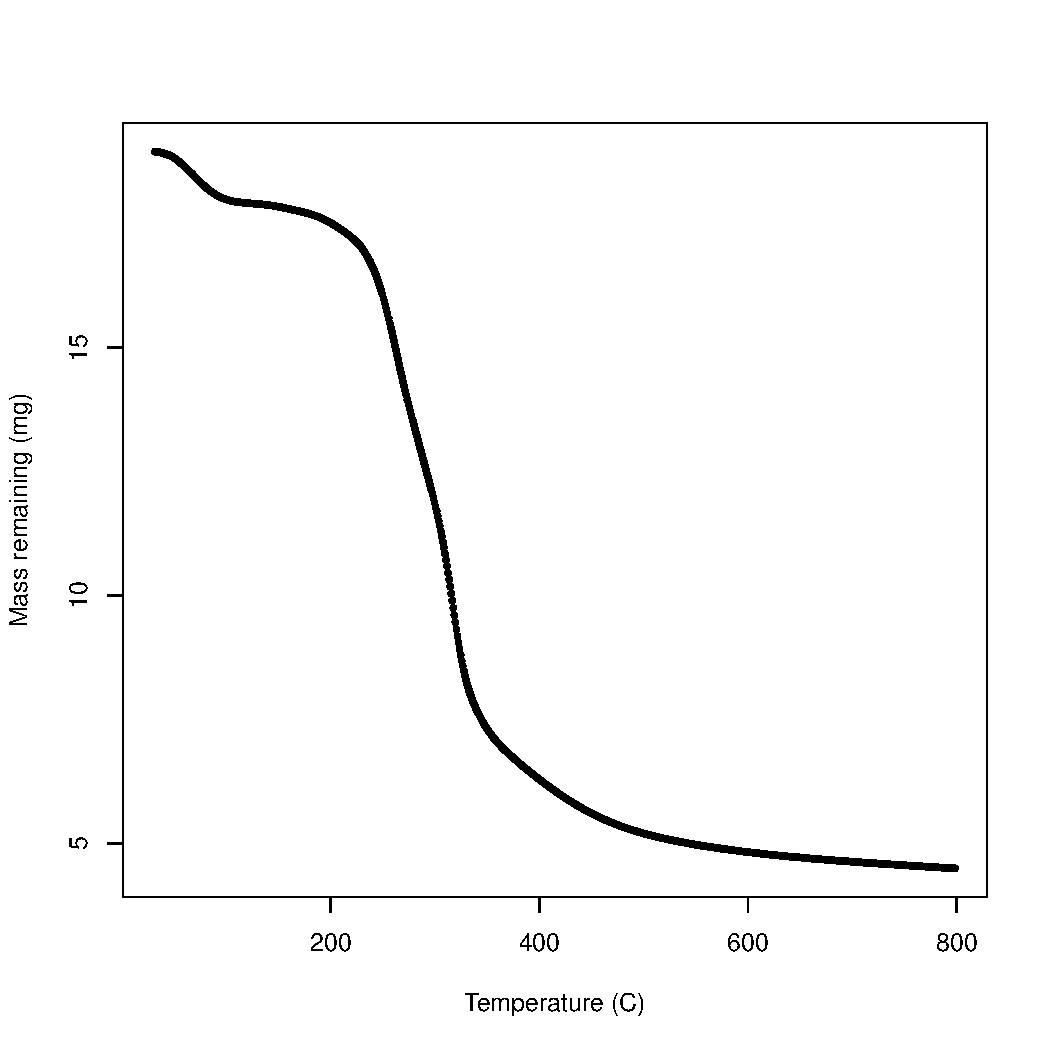
\includegraphics[width=.49\linewidth]{figure/unnamed-chunk-5-1} }
\subfloat[\label{Fig:rateloss} Derivative thermogravimetric rate of mass loss across temperature, scaled by initial mass of sample.\label{fig:unnamed-chunk-52}]{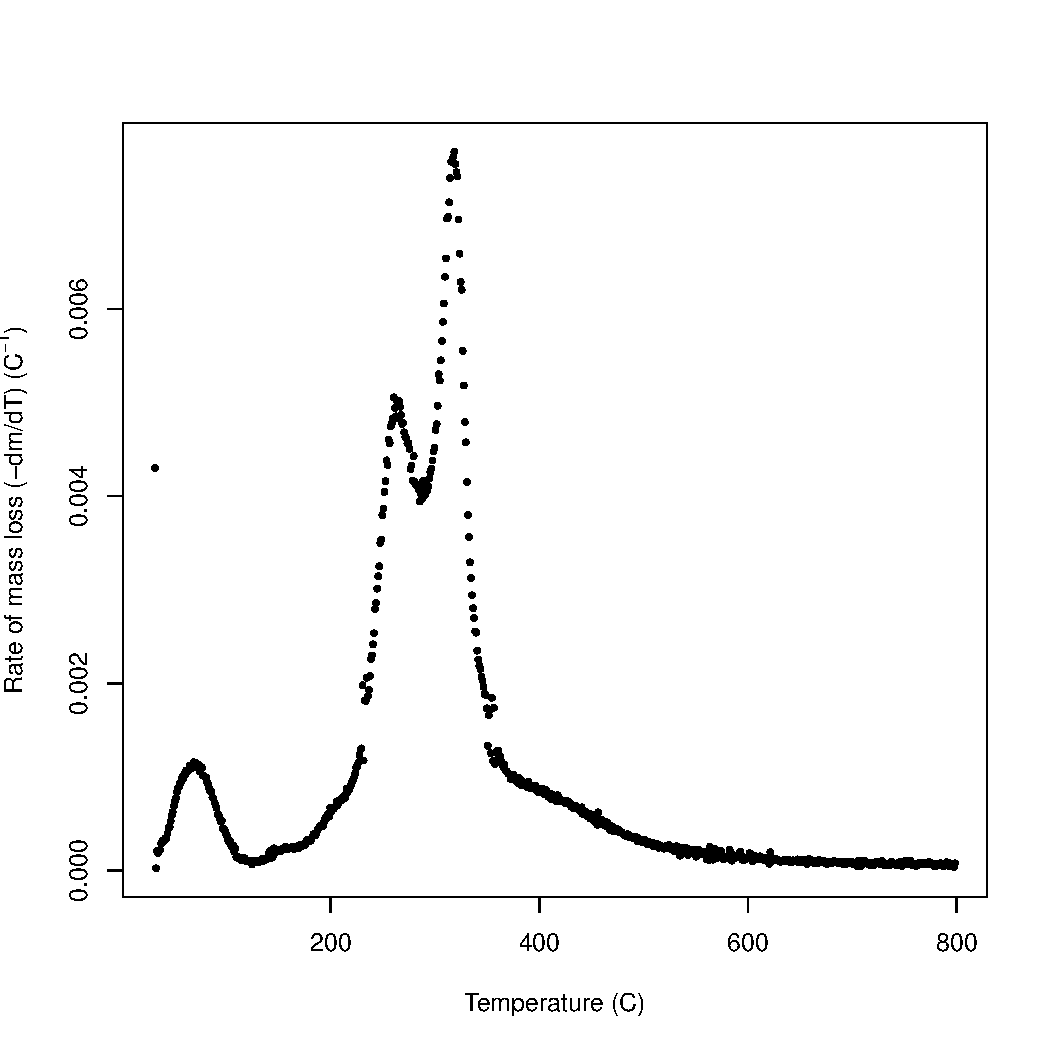
\includegraphics[width=.49\linewidth]{figure/unnamed-chunk-5-2} }\caption{\label{Fig:process} Process function output from \textit{Juncus amabilis} example dataset.}\label{fig:unnamed-chunk-5}
\end{figure}


\end{knitrout}


\begin{table}[!ht]
	\caption{Exported functions}
	\label{Tab:functions}
	\centering
	\footnotesize
	\begin{tabularx}{\linewidth}{llX}
        		\toprule
        		Function family & Function name & Description \\
        		\midrule
		Data & \verb|juncus| & Example thermogravimetric data for \textit{Juncus amabilis} \\
		Data & \verb|marsilea| & Example thermogravimetric data for \textit{Marsilea drumondii} \\
		Basic use & \verb|process()| & Calculates the derivative rate of mass loss of thermogravimetric data \\
		Basic use & \verb|deconvolve()| & Deconvolves derivative rate of mass loss data \\
		Accessor function & \verb|temp_bounds()| & Access temperature bounds used to crop data for mixture model \\
		Accessor function & \verb|rate_data()| & Access processed dataframe including mass loss, rate of mass loss, and temperature \\
		Accessor function & \verb|model_fit()| & Access fit of nonlinear mixture model \\
		Accessor function & \verb|component_weights()| & Access mean, upper, and lower bounds for component weight estimates \\
		Fraser-Suzuki function & \verb|fs_function()| & Fraser-Suzuki equation for a single curve \\
		Fraser-Suzuki function & \verb|fs_mixture()| & Fraser-Suzuki mixture model equation \\
		Fraser-Suzuki function & \verb|fs_model()| & Non-linear model implementation of Fraser-Suzuki mixture model \\
		S3 method & \verb|print(<process>)| & Default print method for process object (derived from \verb|process()|) \\
		S3 method & \verb|plot(<process>)| & Default plot method for process object (derived from \verb|process()|) \\
		S3 method & \verb|print(<deconvolve>)| & Default print method for decon object (derived from \verb|deconvolve()|) \\
		S3 method & \verb|plot(<deconvolve>)| & Default plot method for process object (derived from \verb|deconvolve()|) \\
        		\bottomrule
	\end{tabularx}
\end{table}

\textbf{\textit{Deconvolve data}}\\
Once we have calculated the rate of mass loss, we use the \verb|deconvolve| function to estimate the proportions of carbon components. Under the hood, it does so with a series of steps that are described in detail below. First it crops the derivative rate of mass loss data, then estimates parameter values from the non-linear model, and finally integrates under each resulting curve to estimate weight proportions of primary components. We explain these steps in detail below. \\
\\
\textit{Cropping DTG data}\\
The rate of mass loss (i.e. negative first derivative or DTG) is a multi-peaked curve (Fig.~\ref{Fig:rateloss}) encompassing three main phases \citep{orfao2001}:
\begin{enumerate}
	\item A short period with a pronounced peak of moisture evolution, up until approximately 120 $^{\circ}$C.
	\item A wide mid-range of high mass loss, caused by devolatilisation of primary biomass carbon components, between approximately 120\textendash650 $^{\circ}$C.
	\item A final period of little mass loss when carbonaceous material associated with the inorganic fraction decomposes, after approximately 650 $^{\circ}$C.
\end{enumerate}
Since the overall DTG curve thus represents the loss of extractives, water, inorganic matter, and volatiles in addition to our components of interest \citep{hu2016}, we isolate mass loss from our primary biomass components by cropping the DTG data to Phase 2 (120\textendash650 $^{\circ}$C). The \verb|deconvolve| function defaults to cropping at 120 $^{\circ}$C and 700 $^{\circ}$C, but these can be modified with the \verb|lower_temp| and \verb|upper_temp| arguments.\\
\\
\textit{Non-linear mixture model}\\
Biomass components decompose relatively independently because they do not interact much during thermal volatilisation \citep{yang2006}.
Therefore, the cropped DTG curve can be mathematically deconvolved into constituent parts using a mixture model. The derivative rate of mass loss equation ($\frac{dm}{dT}$) can be expressed as the sum of $n$ independent reactions (Eq.~\ref{eqn:mixture_model}), as follows \citep{orfao2001}:

\begin{align}
	-\frac{dm}{dT} &= \sum\limits_{i=1}^n c_i\frac{d\alpha_{i}}{dT} \label{eqn:mixture_model} \\
	m &= \frac{M_T}{M_0} \label{eqn:fraction} \\
	c_i &= M_{0i} - M_{\infty i} \label{eqn:decayed_mass} \\
	\alpha_i &= \frac{M_{0i} - M_{Ti}}{M_{0i} - M_{\infty i}} \label{eqn:alpha}
\end{align}

where mass ($m$) is expressed as a fraction of mass at temperature $T$ ($M_T$) of the initial sample mass ($M_0$) (Eq.~\ref{eqn:fraction}), $c_i$ is the mass of component $i$ that is decayed (Eq.~\ref{eqn:decayed_mass}), and the mass loss curve of each individual component ($\frac{d\alpha_{i}}{dT}$) is the derivative of $\alpha_i$, the conversion of mass at a given temperature ($M_{Ti}$), from the initial ($M_{0i}$), given total mass lost between the initial and final ($M_{\infty i}$) temperature for each curve  (Eq.~\ref{eqn:alpha}).\\
\\
Although most of our results can be described with only $n = 3$ peaks, corresponding to a single curve each of hemicelluose, cellulose, and lignin, some species yield a second hemicellulose peak at a lower temperature, resulting in $n = 4$ independent curves This is because the soluble carbohydrates in plant tissue can take many forms, including xylan, amylose, etc., which apparently degrade at different temperatures \citep[see also][]{chen2017,muller-hagedorn2007}. \verb|deconvolve| will decide whether three or four curves are best using an internal function that determines if there is a peak below 220 $^{\circ}$C. Upon inspection of your curve you can override this by modifying the \verb|n_curves| argument.\\
\\
In order to fit the mixture model, we must determine the shape of the individual curves ($\frac{d\alpha_{i}}{dT}$) that are summed to produce it. Many different functions have been proposed: the asymmetric bi-Gaussian \citep{sun2015}, logistic \citep{barbadillo2007}, Weibull \citep{cai2007}, asymmetric double sigmoidal \citep{chen2017}, and the Fraser-Suzuki function \citep{perejon2011,hu2016}. Comparisons of several techniques \citep{svoboda2013,perejon2011,cheng2015} found that the Fraser-Suzuki function best fit these kinetic curves, since it allows for asymmetry (a parametric examination of the Fraser-Suzuki function can be found in Fig.~\ref{Fig:fs_simulation}). We therefore use the Fraser-Suzuki function to describe the rate expression of a single curve (Eq.~\ref{eqn:fs_function}) as follows:

\begin{gather}\label{eqn:fs_function}
	\frac{d\alpha_i}{dT} = h_i\ exp\bigg\{-\frac{ln2}{s_i^2}\Big[ln\Big(1 + 2s_i \frac{T - p_i}{w_i}\Big)\Big]^2\bigg\}
\end{gather}

where T is temperature ($^\circ$C), and the parameters $h_i$, $s_i$, $p_i$, and $w_i$ are height, skew, position, and width of the curve, respectively. In total, our model estimates 12 or 16 parameters, one for each parameter of Eq.~\ref{eqn:fs_function} for either 3 or 4 primary components.

\begin{knitrout}\footnotesize
\definecolor{shadecolor}{rgb}{0.969, 0.969, 0.969}\color{fgcolor}\begin{figure}[H]
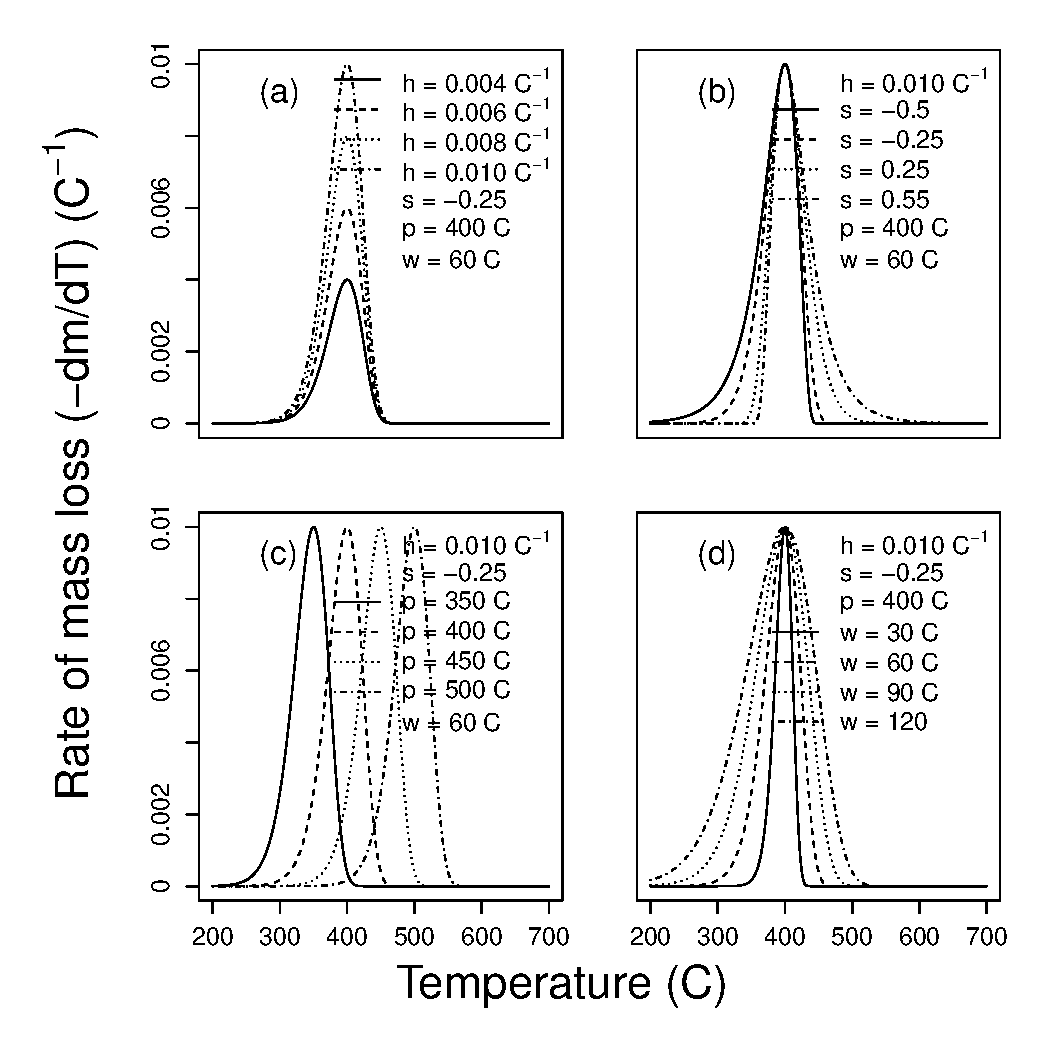
\includegraphics[width=.9\linewidth]{figure/unnamed-chunk-6-1} \caption{\label{Fig:fs_simulation} Parametric examination of Fraser-Suzuki function using simulated data}\label{fig:unnamed-chunk-6}
\end{figure}


\end{knitrout}

\verb|deconvolve| uses non-linear optimisation with residual sum of squares to fit the rate expression \citetext{as in \citealp{cheng2015}}. Starting values were selected based on curves depicted in the literature \citep{muller-hagedorn2007} and from the results of running an identical deconvolution on pure cellulose and lignin samples. Hemicelluloses decay in a reasonably narrow band beginning at a lower temperature \citep{muller-hagedorn2007}, so we used 270 for position and 50 for width. Linear cellulose crystals decay at a higher temperature, but decay more rapidly after peak temperatures are reached, so starting position was set to 310 and width to 30. Lignin typically decays beginning at a high temperature and over a wide interval \citep{chen2015}, so position and width began at 410 and 200, respectively. If necessary, these starting values can also be modified in the \verb|deconvolve| function with the \verb|start_vec|, \verb|lower_vec|, and \verb|upper_vec| arguments. These initial starting values are optimised before model fitting using the \verb|NLOPTR_LN_BOBYQA| algorithm \citep{bobyqa} within the \verb|nloptr| \citep{nloptr} package. Finally, optimised starting values are fit to the non-linear mixture model using \verb|nlsLM()| in the \verb|minpack.lm| \citep{minpack.lm} package.\\
\\
\textit{Component weights}\\
Once overall curve parameters are fit, we can use the pass each components's paremeter estimates to a single Fraser-Suzuki function, and calculate the weight of the component in the overall sample by integrating under the curve (Eq.~\ref{eqn:integration}). To estimate the uncertainty of the weight predictions we calculated the 95\% interval of the weight estimates across a random sample of parameter estimates, drawn in proportion to their likelihood. We assumed a truncated multivariate normal distribution, since the parameters are constrained to positive values, using the modelling package \verb|tmvtnorm| \citep{tmvtnorm}.

\begin{gather}\label{eqn:integration}
	\alpha_i = \int_{120}^{650} h_i\ exp\bigg\{-\frac{ln2}{s_i^2}\Big[ln\Big(1 + 2s_i \frac{T - p_i}{w_i}\Big)\Big]^2\bigg\} dT
\end{gather}

We interpret that the curve located around 250\textendash270 $^\circ$C corresponds to primary hemicelluloses (HC), around 310\textendash330 $^\circ$C to cellulose (CL), and around 330\textendash350 $^\circ$C to lignin (LG). If present, the fourth curve located below 200 $^\circ$C corresponds to the most simple hemicelluloses (HC-1). The second dataset included in the package, \verb|marsilea|, is an example of a four-curve deconvolution. A worked example can be found in the package vignettes.

\begin{knitrout}\footnotesize
\definecolor{shadecolor}{rgb}{0.969, 0.969, 0.969}\color{fgcolor}\begin{kframe}
\begin{alltt}
\hlstd{output_juncus} \hlkwb{<-} \hlkwd{deconvolve}\hlstd{(deriv_juncus)}
\hlstd{output_juncus}
\end{alltt}
\begin{verbatim}
## Deconvolution by 3-part Fraser-Suzuki mixture model fitted to 
## 580 datapoints from 120 to 700 degrees C.
\end{verbatim}
\end{kframe}
\end{knitrout}

The output of the \verb|deconvolve| function is a list of five items:
\begin{enumerate}
\item{the data used to fit the function,
\begin{knitrout}\footnotesize
\definecolor{shadecolor}{rgb}{0.969, 0.969, 0.969}\color{fgcolor}\begin{kframe}
\begin{alltt}
\hlstd{DTG_data} \hlkwb{<-} \hlkwd{rate_data}\hlstd{(output_juncus)}
\hlkwd{head}\hlstd{(DTG_data)}
\end{alltt}
\begin{verbatim}
##       temp_C        deriv   mass_T
## 5325 120.514 9.570652e-05 17.91630
## 5384 121.501 9.885901e-05 17.91445
## 5445 122.515 1.003878e-04 17.91252
## 5505 123.514 9.133606e-05 17.91079
## 5565 124.513 6.493836e-05 17.90956
## 5625 125.509 8.578618e-05 17.90794
\end{verbatim}
\end{kframe}
\end{knitrout}
}
\item{the upper and lower temperature bounds to which the data were cropped,
\begin{knitrout}\footnotesize
\definecolor{shadecolor}{rgb}{0.969, 0.969, 0.969}\color{fgcolor}\begin{kframe}
\begin{alltt}
\hlkwd{temp_bounds}\hlstd{(output_juncus)}
\end{alltt}
\begin{verbatim}
## [1] 120 700
\end{verbatim}
\end{kframe}
\end{knitrout}

}
\item{the model fit including parameter estimates,
\begin{knitrout}\footnotesize
\definecolor{shadecolor}{rgb}{0.969, 0.969, 0.969}\color{fgcolor}\begin{kframe}
\begin{alltt}
\hlkwd{model_fit}\hlstd{(output_juncus)}
\end{alltt}
\end{kframe}
\end{knitrout}

\begin{knitrout}\footnotesize
\definecolor{shadecolor}{rgb}{0.969, 0.969, 0.969}\color{fgcolor}\begin{kframe}
\begin{verbatim}
## Nonlinear regression model
##   model: deriv ~ fs_mixture(temp_C, height_1, skew_1, position_1,
##     width_1, height_2, skew_2, position_2, width_2, height_3,
##     skew_3, position_3, width_3)
##   data: dataframe
##   height_1   skew_1     position_1 width_1    height_2   skew_2
##   3.944e-03  1.258e-01  2.662e+02  5.106e+01  5.793e-03  1.344e-02
##   position_2 width_2    height_3   skew_3     position_3 width_3
##   3.173e+02  2.866e+01  1.163e-03  1.085e-01  3.300e+02  2.500e+02
##   residual sum-of-squares: 9.299e-06
## 
## Number of iterations to convergence: 23
## Achieved convergence tolerance: 1.49e-08
\end{verbatim}
\end{kframe}
\end{knitrout}
}
\item{the number of curves,
\begin{knitrout}\footnotesize
\definecolor{shadecolor}{rgb}{0.969, 0.969, 0.969}\color{fgcolor}\begin{kframe}
\begin{alltt}
\hlstd{output_juncus}\hlopt{$}\hlstd{n_curves}
\end{alltt}
\begin{verbatim}
## NULL
\end{verbatim}
\end{kframe}
\end{knitrout}
}
\item{and the mean and upper and lower estimates of the weight of each component.
\begin{knitrout}\footnotesize
\definecolor{shadecolor}{rgb}{0.969, 0.969, 0.969}\color{fgcolor}\begin{kframe}
\begin{alltt}
\hlkwd{component_weights}\hlstd{(output_juncus)}
\end{alltt}
\begin{verbatim}
##   HC CL LG value_type
## 1  0  0  0       2.5%
## 2  0  0  0      97.5%
## 3  0  0  0       mean
\end{verbatim}
\end{kframe}
\end{knitrout}
}
\end{enumerate}
If you \verb|plot()| the output of the \verb|deconvolve| function you will see the result of the deconvolution (Fig.~\ref{Fig:decon}). This default plot shows the underlying DTG data, the overall mixture model curve, as well as the components curves.

\begin{knitrout}\footnotesize
\definecolor{shadecolor}{rgb}{0.969, 0.969, 0.969}\color{fgcolor}\begin{kframe}
\begin{alltt}
\hlkwd{plot}\hlstd{(output_juncus)}
\end{alltt}
\end{kframe}\begin{figure}[H]
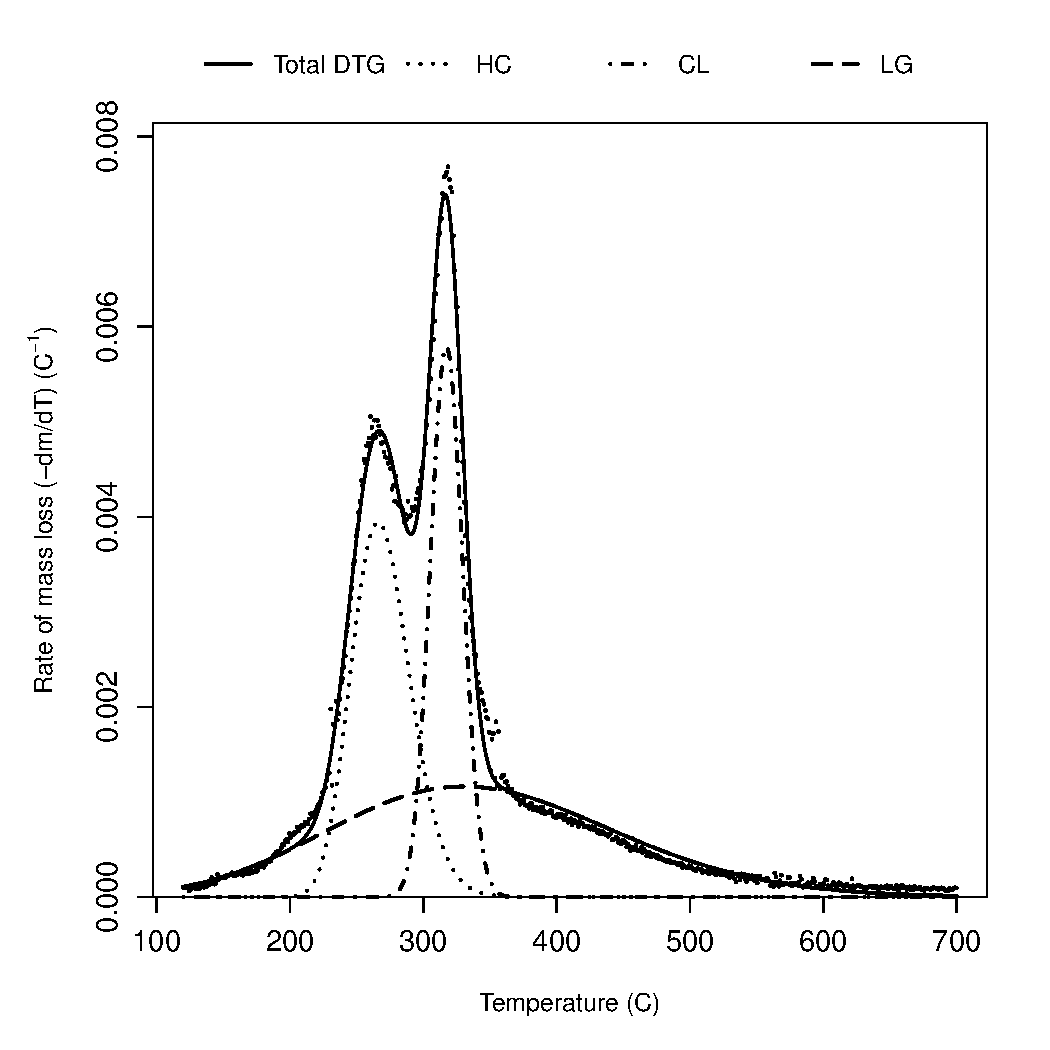
\includegraphics[width=\maxwidth]{figure/unnamed-chunk-14-1} \caption{\label{Fig:decon} Deconvolution of 	extit{Juncus amabilis} example dataset. Mass loss data overlaid with output of deconvolution. Rate of mass loss scaled by initial mass of sample.}\label{fig:unnamed-chunk-14}
\end{figure}


\end{knitrout}

All analyses were conducted within the statistical computing environment, R \citep{R}, and data and R code for this paper are available on the package Github (\url{https://github.com/smwindecker/deconvolve/}. In order to aid in the reproducibility of this work, our code was written using a \verb|remake| framework \citep{remake}. This allows others to readily reproduce our work by calling \verb|remake()| in R.


This work is the first attempt to use thermogravimetric analysis (TGA) with a mixture model to estimate the partitioning of carbon in a suite of wetland plants.



\section*{Quality control}
All the functions of \verb|deconvolve| were tested to see if they produced the desired output. ?... The structure of the package successfully passed the \verb|CRAN R CMD| check and the results from this check can be found on CRAN.

\section*{(2) Availability}
\vspace{0.5cm}
\section*{Operating system}
The package can work with either Windows, Mac OS X, or Linux.

\section*{Programming language}
R version XXX or higher.

\section*{Additional system requirements}
An internet connection is required to install the \verb|deconvolve| package.

\section*{Dependencies}
R packages: \verb|graphics|, \verb|minpack.lm|, \verb|nloptr|, \verb|stats|, \verb|tmvtnorm|, \verb|zoo|.

\section*{List of contributors}
This package was created by Saras Windecker and Dr. Nick Golding.

\section*{Software location:}

{\bf Archive} (e.g. institutional repository, general repository) (required – please see instructions on journal website for depositing archive copy of software in a suitable repository)

\begin{description}[noitemsep,topsep=0pt]
	\item[Name:] The name of the archive.
	\item[Persistent identifier:] e.g. DOI, handle, PURL, etc.
	\item[Licence:] Open license under which the software is licensed.
	\item[Publisher:] Name of the person who deposited the software.
	\item[Version published:] The version number of the software archived.
	\item[Date published:] dd/mm/yy
\end{description}


{\bf Code repository} GitHub

\begin{description}[noitemsep,topsep=0pt]
	\item[Name:] \url{https://github.com/smwindecker/deconvolve/}
	\item[Persistent identifier:] e.g. DOI, handle, PURL, etc.
	\item[Licence:] Open license under which the software is licensed.
	\item[Date published:] dd/mm/yy
\end{description}

\section*{Language}
R

\section*{(3) Reuse potential}
This should include the use cases for the software,

The Fraser-Suzuki family of functions are exported to allow the user to create their own plots from the model outputs. Detailed descriptions of how to do so are included in the package vignettes.

This package was designed with both the user and developer in mind. There are several vignettes available with the package and on the package website (\url{https://smwindecker.github.io/deconvolve/}) facilitating exploration of package functionality. For those that wish to contribute to the package, it is hosted on Github, and they can log issues via the issues tracker (\url{https://github.com/smwindecker/deconvolve/issues}) or submit a pull request to add functionality to the package.

\section*{Acknowledgements}
The authors would like to thank Dr. Nick Tierney for reviewing an early version of the package. We would like to thank the University of Melbourne Department of Chemical and Biomolecular Engineering for access to and training on the TGA-FTIR. Vegetation collection for data used to build and verify the model was conducted under Victorian Department of Environment, Land, Water and Planning Permit No 10007429. We would like to thank volunteers Paula Sanchez, Abbey Kinnish, Kelsey Johnson, Madeline Brenker, and Urtzi Enriquez Urzelai for assistance in the field collecting plant specimens.

\section*{Funding statement}
The authors would like to acknowledge support from the Australian Research Council Centre of Excellence for Environmental Decisions, the Holsworth Wildlife Reseach Endowment \& The Ecological Society of Australia, and the Melbourne International Research Scholarship and Melbourne International Fee Remission Scholarship from University of Melbourne.

\section*{Competing interests}
The authors declare that they have no competing interests.

\section*{References}
\bibliography{bibliography_papers,bibliography_packages}

\vspace{2cm}

\end{document}
